\subsection{Scaling Violations in parton densities}

QCD introduces a \(Q^2\) dependence into the parton distribution functions which is calculable using the evolution equations
%
\begin{eqnarray}
  \frac{d~\Delta q(x,Q^2)}{d~ln Q^2} &=& \frac{\alpha_s}{2 \pi} \left[ \Delta P_{qq} \otimes \Delta q + \Delta P_{qg} \otimes \Delta g \right] \nonumber \\
  \frac{d~\Delta g(x,Q^2)}{d~ln Q^2} &=& \frac{\alpha_s}{2 \pi} \left[ \Delta P_{gq} \otimes \Delta q + \Delta P_{gg} \otimes \Delta g \right].
\end{eqnarray}
%
The \(\Delta P\) are polarized splitting functions calculated perturbatively in \(\alpha_s\).  The original parton model equation for \(g_1\) \ref{eqn:simple-g1} becomes
%
\begin{equation}
  g_1(x, Q^2) = \frac{1}{2} \sum_{j} e_j^2 \left[\Delta q_j^2 + \Delta \bar{q}_j^2 + \frac{\alpha_s}{2 \pi} \left(\Delta C_j \otimes \left[\Delta q_j + \Delta \bar{q}_j\right] + \Delta C_g \otimes \Delta g\right)\right].
  \label{eqn:enhanced-g1}
\end{equation}
%
where the sum is over flavors and the \(\Delta C_j\) are Wilson coefficients. Given measurements of \(g_1\) at a fixed value of \(x\) and varying \(Q^2\), one can use \ref{eqn:enhanced-g1} to solve for the polarized gluon density. The  technique has proven very effective in unpolarized DIS, where precise measurements of the structure functions across five decades in \(Q^2\) yield an excellent ``lever arm''.  In contrast, Figure \ref{fig:g1-versus-q2} plots the world data on \(g_1\).  Extractions of \(\Delta g(x)\) from these data are prone to significant uncertainties.  An example analysis from Leader, Sidorov, and Stamenov is shown in Figure \ref{fig:g1-deltag}; in that analysis, even the sign of the gluon polarization is not constrained by the data.

\begin{figure}
  \centering
  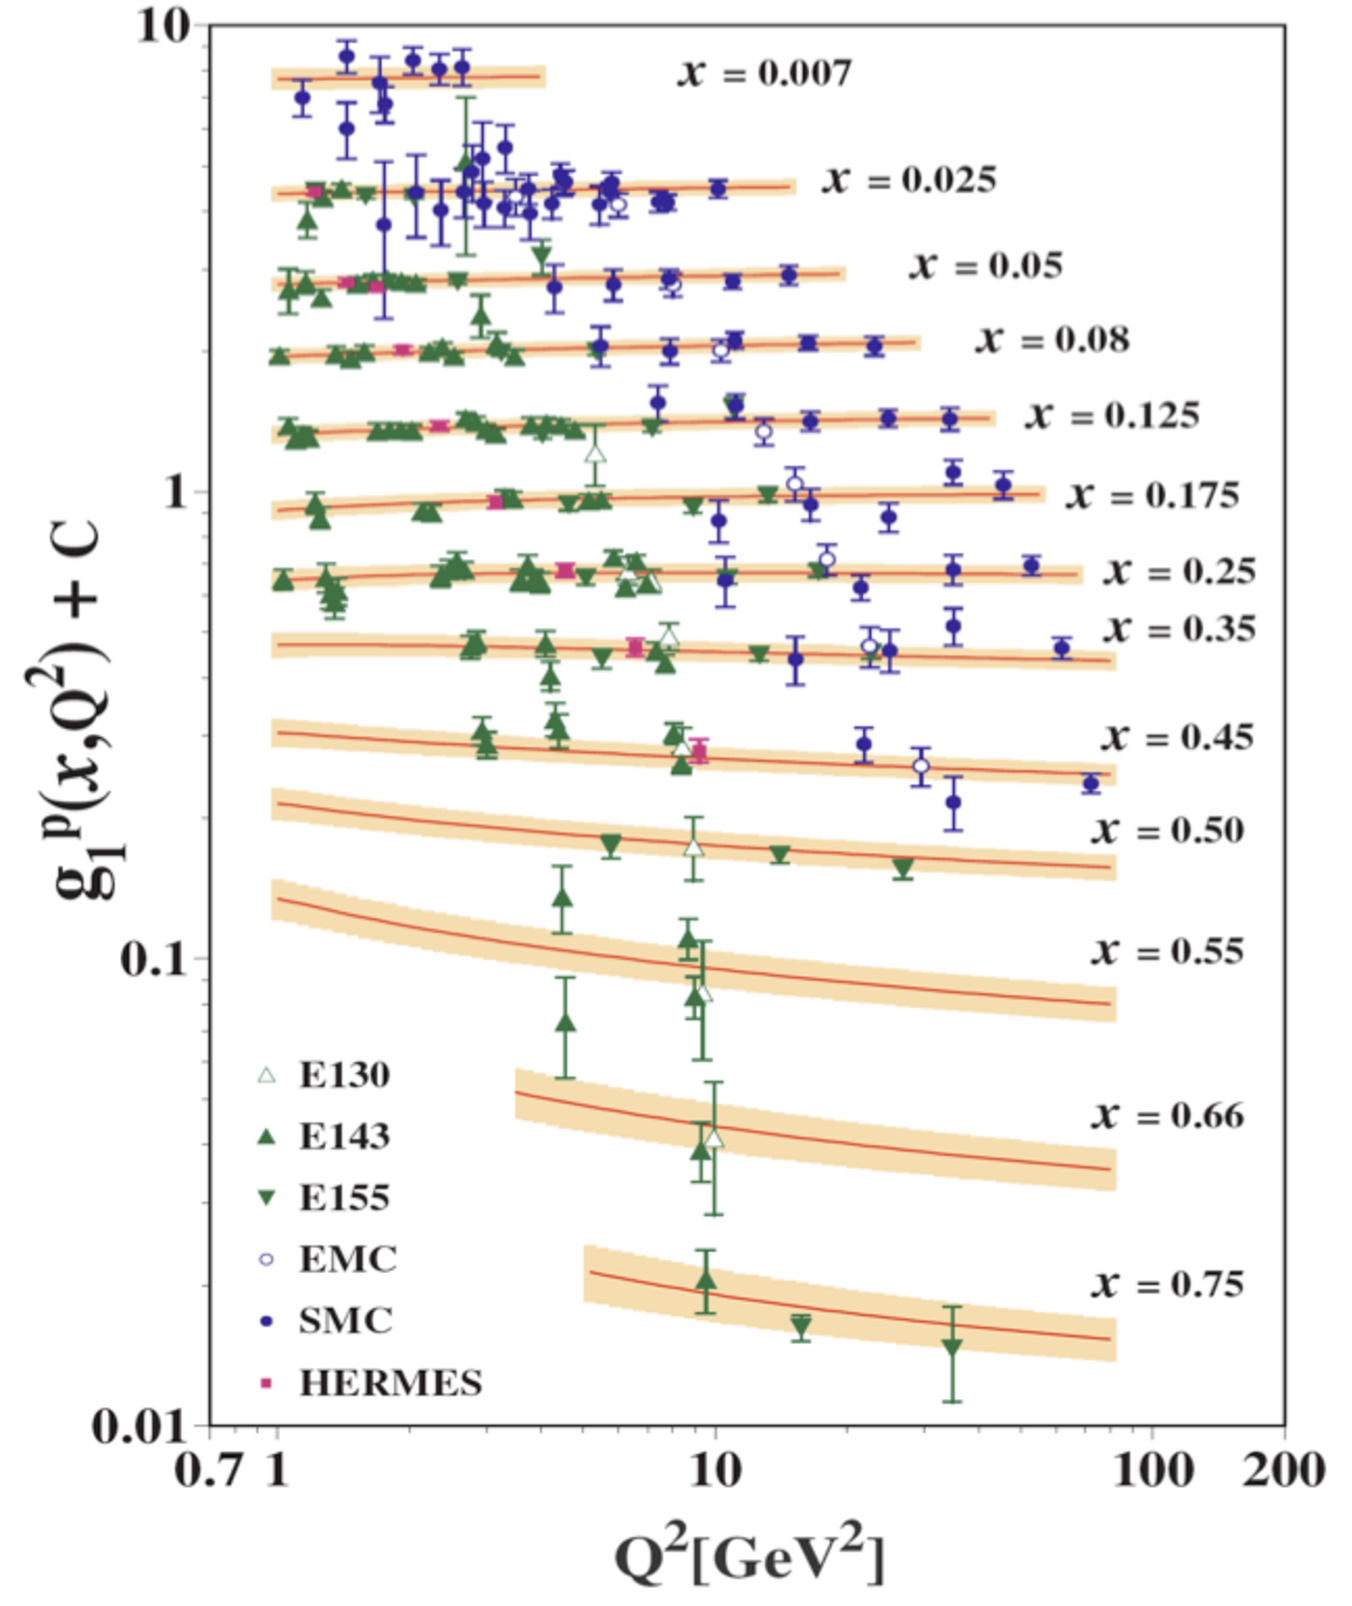
\includegraphics[width=0.7\textwidth]{figures/g1_x_q2}
  \caption{World data on the $g_1$ structure functions of the proton, plotted
  versus $Q^2$ for several values of $x$. An analysis of the variation with
  $Q^2$ yields a parameterization of the polarization gluon distribution.}
  % http://www2.lns.mit.edu/eic/Bruell.pdf
  \label{fig:g1-versus-q2}
\end{figure}

\begin{figure}
  \centering
  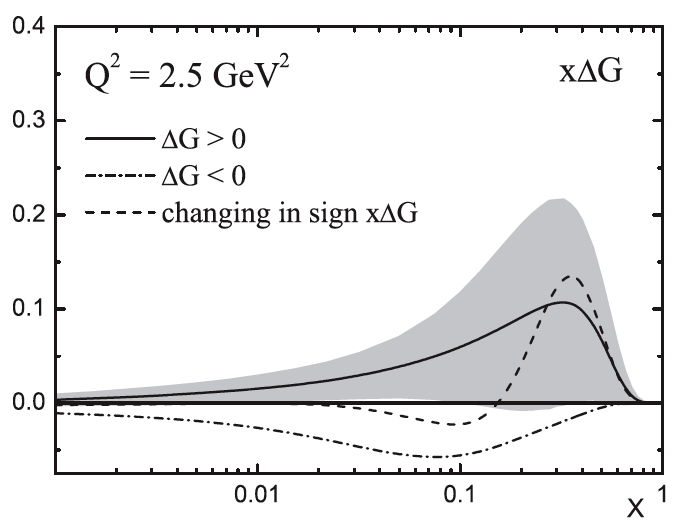
\includegraphics[width=0.6\textwidth]{figures/lss06_deltag}
  \caption{Extraction of the polarized gluon distribution from an analysis of
  scaling violations in DIS and SIDIS. The gray band indicates statistical and
  systematic uncertainties summed in quadrature. Analyses assuming positive,
  negative, and sign-changing gluon polarization all resulted in a comparable
  goodness-of-fit \cite{Leader:2006xc}}
  \label{fig:g1-deltag}
\end{figure}
